\documentclass[11pt,a4paper]{article}
\usepackage[margin=2.4cm]{geometry}
\usepackage{graphicx}
\usepackage{amsmath}
\usepackage{amssymb}
\usepackage{xcolor}
\usepackage[colorlinks=true,linkcolor=blue!50!black,urlcolor=blue!50!black,citecolor=blue!50!black]{hyperref}
\graphicspath{{figs/}}

\newcommand{\He}[1]{$^{#1}$He}
\newcommand{\sM}{\sigma_{\mathrm{M1}}}
\newcommand{\sE}{\sigma_{\mathrm{E0}}}
\newcommand{\En}{E_n}

\title{\vspace{-1.2cm}
  {\Large\bfseries The final metric: X17 / IPC pairs vs neutron energy,
   with the $\gamma$-dark E0 channel and the trigger window}\\[2mm]
  {\large Folding formation $\times$ pair-fraction $\times$ acceptance
   $\times$ readout time into recorded pairs per day}}
\author{Dylan Neff}
\date{15 June 2026 \\[2mm]
  {\small\itshape Internal note --- informal. Drafted by Claude (Anthropic AI
  assistant) under D.~Neff's direction; \\ physics, numbers and text
  reviewed by D.~Neff.}}

\begin{document}
\maketitle
\vspace{-0.8cm}

%=============================================================================
\section*{Part 0 --- Summary}

\begin{center}
\fcolorbox{blue!40!black}{blue!4}{%
\begin{minipage}{0.95\textwidth}
\vspace{3pt}
This note finishes the E0 thread: it turns the settled \emph{shapes}
(formation $\times$ decay, the previous note) into the \textbf{recorded} metric
--- X17 and IPC $e^+e^-$ pairs per day vs neutron energy --- by folding in the
absolute campaign normalisation, the detector acceptance, and (the decisive new
ingredient) \textbf{the trigger/readout time window}.
\begin{itemize}\setlength\itemsep{1pt}
  \item \textbf{Two pair families, opposite energy ends, opposite triggers.}
    M1/E1 IPC pairs ride the rising radiative capture $\Rightarrow$ peak at MeV
    ($\En\gtrsim100$\,keV); the $\gamma$-dark E0 pairs sit \textbf{sub-keV}.
  \item \textbf{The flash readout cannot see E0.} At $L=19.5$\,m the
    $\sim$10\,\textmu s flash readout reaches only $\En\gtrsim20$\,keV; the E0
    pairs (sub-keV, TOF $>45$\,\textmu s) arrive \emph{after} it closes.
    Recorded E0 in the flash window $\approx0$.
  \item \textbf{Only a thermal trigger records E0} --- and even then it is
    small: with $f=\sE/\sM\le10^{-2}$, the E0 channel yields
    $\lesssim$3 IPC background pairs/day and $\lesssim$0.06 X17/day recorded,
    because the E0 capture inherits the same tiny radiative branching
    ($\sigma_{n\gamma}/\sigma_{np}\sim10^{-8}$) that kills the whole sub-keV
    program, times $f$.
  \item \textbf{Headline (flash readout, the baseline run):}
    $\sim$500 IPC background pairs/day and \textbf{$\sim$6--10 X17/day}
    recorded (table vs anchored $\alpha_{\rm IPC}$), \emph{all from M1/E1};
    E0 adds nothing here. This reproduces the committed numbers
    ($\sim$190 X17 / 30-day run).
  \item \textbf{E0 \emph{does} make X17} if X17 is a massive vector or scalar
    (it is not $\gamma$-dark to a massive boson) --- but the rate is tiny
    because the E0 \emph{capture} is tiny. \textbf{Bottom line: including E0 is
    a model-completeness improvement, not a game-changer for the measurement.}
\end{itemize}
\vspace{3pt}
\end{minipage}}
\end{center}

%=============================================================================
\section{The metric, assembled}

The previous note settled, vs neutron energy, \emph{which} \He{4}$^*$ state
forms (Part 1, the shape) and \emph{whether it makes a pair} (Part 2, the
height). Here we evaluate
\[
N_{\rm rec}(\En)=\underbrace{\Big[\,N_{\rm M1/E1}(\En)+N_{\rm E0}(\En;f)\,\Big]}
   _{\text{produced / pulse}}\times\;
   \underbrace{A}_{\text{acceptance}}\times\;
   \underbrace{T(\En)}_{\text{TOF window}},
\]
summed over decades and $\times$ pulses/day. The four ingredients, with their
sources:
\begin{itemize}\setlength\itemsep{1pt}
  \item \textbf{M1/E1 (term 1):} $N_{\rm M1/E1}=N_{n\gamma}^{\rm direct}(\En)\,
    \alpha_{\rm IPC}$, the \emph{directly counted} 714 \He{3}$(n,\gamma)$\He{4}
    events per decade from the $5\times10^{8}$-neutron campaign
    (\texttt{mev\_rates.json}), times the high-energy IPC coefficient
    $\alpha_{\rm IPC}$. With the table $\alpha=2.1\times10^{-3}$ this
    reproduces the committed MeV-note budget exactly (32.7 X17/day produced).
    The $^{12}$C/$^8$Be-anchored $\alpha=3.5\times10^{-3}$ is used as the
    default ($\times1.67$).
  \item \textbf{E0 (term 2):} $N_{\rm E0}=N_{np}(\En)\,f\,
    (\sigma_{n\gamma}/\sigma_{np})_{\rm th}\,g_{0^+}(\En)$, the sub-threshold
    $0^+$ construction of the previous note (\texttt{make\_e0\_pair\_yield\_fig.py}),
    carried over the bracket $f=10^{-3}$--$10^{-2}$.
  \item \textbf{Acceptance $A$:} flat MM-double geometric acceptance from the
    $10^{7}$-event at-rest \texttt{pairs\_v2} study --- \textbf{19.6\,\% (X17),
    23.6\,\% (IPC)} (angular-resolution note). Energy-independent; the E0
    monopole pair kinematics differ slightly (caveat below).
  \item \textbf{Trigger window $T(\En)$:} TOF$(\En)=L/v$, $L=19.5$\,m.
    The flash readout ($\sim$10\,\textmu s) accepts $\En\gtrsim20$\,keV; a
    \textbf{thermal trigger} recovers the sub-keV decades. We tabulate both.
\end{itemize}

%=============================================================================
\section{The money table}

\begin{center}
\renewcommand{\arraystretch}{1.2}
\begin{tabular}{lrrr}
\hline
per day & produced & recorded, & recorded, \\
($\alpha_{\rm IPC}=3.5\times10^{-3}$) & & flash 10\,\textmu s & flash $+$ thermal \\
\hline
\multicolumn{4}{l}{\emph{IPC background pairs}}\\
\quad M1/E1               & $2182$ & $504$ & $515$ \\
\quad E0, $f=10^{-3}$     & $1.3$  & $0.02$ & $0.30$ \\
\quad E0, $f=3\times10^{-3}$ & $3.9$ & $0.05$ & $0.91$ \\
\quad E0, $f=10^{-2}$     & $12.9$ & $0.15$ & $3.0$ \\
\hline
\multicolumn{4}{l}{\emph{X17 signal}}\\
\quad from M1            & $54.5$ & $10.5$ & $10.7$ \\
\quad from E0, $f=10^{-3}$ & $0.03$ & $0.00$ & $0.01$ \\
\quad from E0, $f=10^{-2}$ & $0.32$ & $0.00$ & $0.06$ \\
\hline
\end{tabular}
\end{center}

\noindent With the table $\alpha=2.1\times10^{-3}$ every M1/E1 and X17-from-M1
row scales by $0.6$: produced X17 from M1 $=32.7$/day, \textbf{recorded
(flash) $=6.3$/day} ($\approx$190 per 30-day run) --- the committed baseline.
The X17-from-E0 rows assume the E0 $\to$ X17 branching equals the M1 value
(2.5\,\% per pair) as a \emph{benchmark}; see \S4.

%=============================================================================
\section*{}
\begin{center}
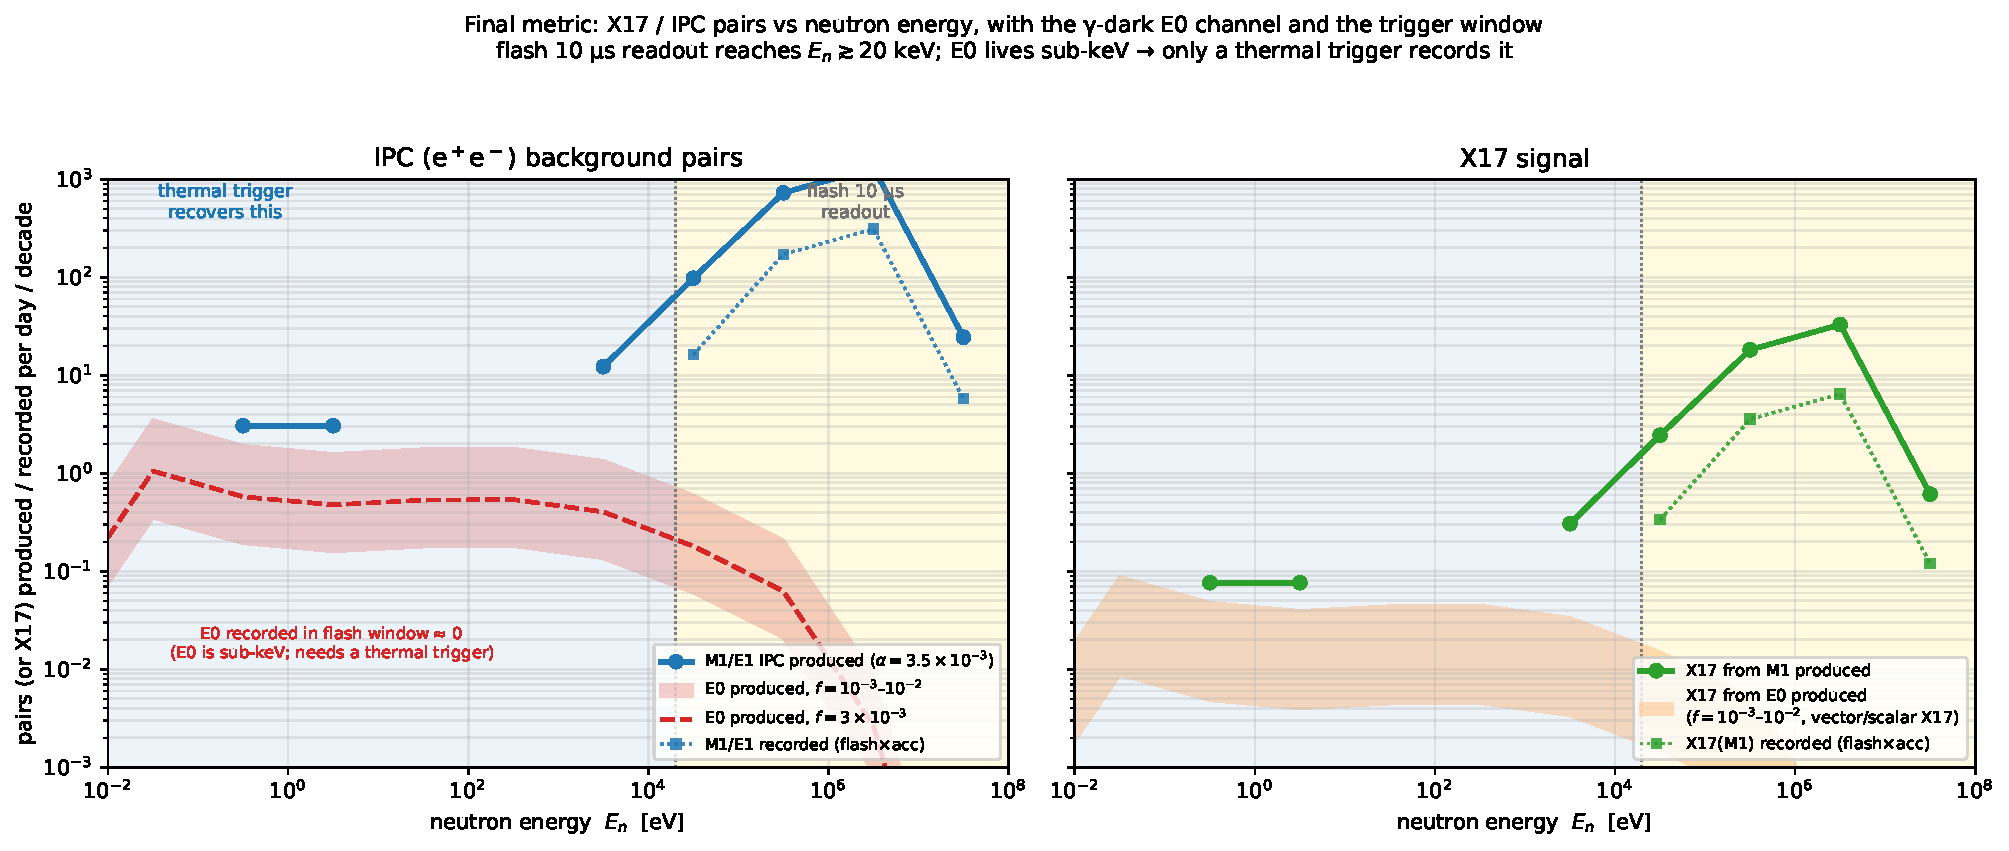
\includegraphics[width=0.99\textwidth]{fig_e0_final_metric.pdf}
\end{center}
\noindent \textbf{Left:} IPC background pairs/day per decade. M1/E1 (blue) peaks
at MeV and is what the flash readout records (dotted, $\En\gtrsim20$\,keV); the
E0 band (red, $f=10^{-3}$--$10^{-2}$) lives sub-keV, in the region only a
thermal trigger reaches. \textbf{Right:} the X17 signal --- from M1 (green) and,
if X17 is a massive vector/scalar, from E0 (orange band). The gold/blue shading
marks the flash-window vs thermal-trigger energy regions, split at 20\,keV.

%=============================================================================
\section{Does E0 make X17? Yes, if X17 is massive vector or scalar}

The reason $0^+\!\to0^+$ is $\gamma$-dark is specifically that \textbf{the photon
is massless} --- it has only transverse polarisations and cannot carry off a
monopole. That is exactly why E0 instead proceeds through a \emph{virtual}
(longitudinal) photon: internal conversion and internal pair creation. \textbf{X17
is massive} ($\sim$17\,MeV), so the argument that kills the photon does not kill
X17. Working through the two-body $0^+\!\to0^++X$ selection rules:

\begin{center}
\renewcommand{\arraystretch}{1.15}
\begin{tabular}{lcl}
\hline
X17 hypothesis & $J^P$ & $0^+\!\to0^+$ emission \\
\hline
vector (dark photon) & $1^-$ & \textbf{allowed} ($L=1$) \\
scalar               & $0^+$ & \textbf{allowed} ($L=0$) \\
pseudoscalar         & $0^-$ & forbidden \\
axial-vector         & $1^+$ & forbidden \\
\hline
\end{tabular}
\end{center}

\noindent So for the usually-assumed vector (dark-photon) X17 the monopole
channel is open: \textbf{E0 is $\gamma$-dark but \emph{not} X17-dark}, and could
even be relatively \emph{enhanced} (X17 is not competing against the 0.35\,\%
IPC tail of a real $\gamma$, the same logic that makes E0 ``100\,\% pairs'').
Two honest caveats keep this from being a discovery:
\begin{enumerate}\setlength\itemsep{1pt}
  \item The E0$\to$X17 branching is a \emph{separate} unknown --- not the
    2.5\,\% measured for the M1 line (different multipole, phase space,
    coupling). The table uses 2.5\,\% only as a placeholder.
  \item Whatever the branching, the rate is bounded by the E0 \emph{capture}
    rate, which is small ($\le13$ pairs/day produced even at $f=10^{-2}$). So
    X17-from-E0 is $\lesssim$0.3/day produced, $\lesssim$0.06/day recorded.
\end{enumerate}

%=============================================================================
\section{What this means for the measurement}

\begin{itemize}\setlength\itemsep{2pt}
  \item \textbf{The flash-readout run is unaffected by E0.} Its $\sim$6--10
    recorded X17/day and $\sim$500 IPC background pairs/day are entirely M1/E1;
    E0 contributes $<0.2$/day because it is sub-keV and arrives after the
    window. Leaving E0 out of the generator does \emph{not} bias the baseline
    high-energy analysis.
  \item \textbf{A thermal trigger is the only way to reach E0}, and the prize is
    modest: $\le3$ extra IPC background pairs/day and $\le0.06$ X17/day, sitting
    on the enormous sub-keV charged-particle load ($\sim3\times10^{5}$ (n,p)t
    per pulse in the opaque gas). The statistics exist in \emph{thermals}, but
    the E0 pair signal is $f\times10^{-8}$ of them --- S/B is the obstacle, not
    rate. A thermal trigger is still worth scoping, but E0 alone does not
    motivate it.
  \item \textbf{Generator action item is small and low-priority.} If we add E0
    for completeness, it is a third pair sub-generator at the $0^+$ transition
    energy with monopole kinematics, weighted by $N_{\rm E0}/N_{\rm M1/E1}$; it
    will not move the recorded spectra under the flash readout.
\end{itemize}

\subsection*{Caveats}
Acceptance is the flat at-rest geometric value; the E0 monopole opening-angle
distribution differs from the E1/IPC one the response was built on, so the E0
acceptance is approximate (the rate conclusion is robust to it). $f$ remains
bracketed, not pinned --- a \He{4} R-matrix normalised by the $(e,e')$ monopole
strength is still the way to a number. All MeV-region numbers are at-rest
kinematics; the $\En$-dependent boost ($E^*=20.58+\tfrac34\En$) shifts the
\emph{shapes} but not these integrated rates.

%=============================================================================
\section*{Reproducing this note}
{\raggedright
\texttt{scripts/make\_e0\_final\_metric.py} reads
\texttt{analysis/mev/mev\_rates.json} and \texttt{data/He3.h5}, writes
\texttt{docs/report/figs/fig\_e0\_final\_metric.\{pdf,png\}} and the table
numbers to \texttt{analysis/e0/final\_metric.json}. Inputs trace to the MeV
campaign (\texttt{mev\_note.tex}), the angular-resolution acceptance
(\texttt{docs/angular\_resolution/}), and the E0 physics
(\texttt{docs/e0\_branch/}, \texttt{e0\_pair\_channel\_note.tex}).
\par}

\end{document}
